\section{Sistemi bifase}

Le grandezze estensive specifiche sono la media pesata sulle masse:
\[m = m_\alpha + m_\beta \qquad E = E_\alpha + E_\beta\]
\[e = \frac{m_\alpha}{m}e_\alpha + \frac{m_\beta}{m}e_\beta\]
\[\text{frazione massica:} \quad x_\alpha = \frac{m_\alpha}{m} \quad x_\beta = \frac{m_\beta}{m} \]

Dalla regola di Gibbs il numero di variabili intensive indipendenti per bifase monocomponente è 1, pressione e temperatura non sono indipendenti. Lo stato termodinamico è descritto da una coppia intensiva-estensiva oppure da una coppia estensiva-estensiva.

Per un sistema monocomponente trifase, sempre secondo la regola di Gibbs le variabili intensive indipendenti sono 0, lo stato termodinamico è descritto da una coppia estensiva-estensiva.

\subsection{Stati di aggregazione}
\begin{tabular}{p{2.7cm}p{4.5cm}}
    Liq. sottoraffreddato & Non in procinto di evaporare \\
    Liq. saturo & In procinto di evaporare \\
    Vapore umido & Stato di transizione \\
    Vapore saturo & In procinto di condensazione \\
    Vapore surriscaldato & Non in procinto di condensazione \\
\end{tabular}

\subsection{Diagramma di stato P-v-T}

\begin{center}
    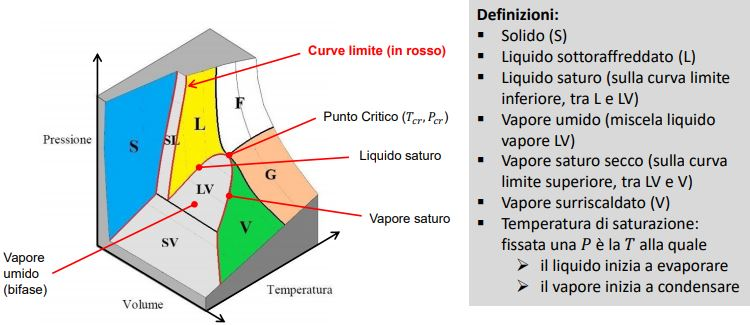
\includegraphics[height=3cm]{Diagramma di stato P-v-T.JPG}
\end{center}


\subsection{Entalpia (calore) di transizione}
La transizione di fase è a P costante: $\dd{h} = \delta q$ (calore necessario = entalpia di transizione).

\[ h_\text{solido} < h_\text{liquido} < h_\text{vapore} \]

Per l'acqua allo stato triplo:
\begin{tabular}{ll}
    Solidificazione & $h_{lst,\ch{H2O}} = \SI{-333}{kJ/Kg}$ \\
    Evaporazione & $h_{lvt,\ch{H2O}} = \SI{2501.6}{kJ/Kg}$
\end{tabular}

\subsection{Titolo di vapore, liquido e solido}
\[ x = x_v = \frac{m_v}{m} \quad x_l = \frac{m_l}{m} \quad x_s = \frac{m_s}{m} \]
\[ x_v + x_l + x_s = 1 \]

Per interpolare lineare nelle tabelle:
\[ Y = Y_A + \frac{Y_B-Y_A}{X_B-X_A}(X-X_A) \]
$Y$: grandezza che si vuole calcolare \newline
$X$: grandezza conosciuta \newline
$A, B$: stati di riferimento (presenti in tabella) con $X_A < X < X_B$ \newline
oppure
\[ \frac{X-X_1}{X_2-X_1} = \frac{T-T_1}{T_2-T_1} \]
\ \newline \newline
Per interpolare bilinearmente nelle tabelle:
\[ Y = Y_A + \frac{Y_B-Y_A}{X_B-X_A}(X-X_A) \]
con
$Y_A = Y_{A1} + \frac{Y_{A2} - Y_{A1}}{X_{A2 - X_{A1}}}(X_A-X_{A1})$
$Y_B = Y_{B1} + \frac{Y_{B2} - Y_{B1}}{X_{B2 - X_{B1}}}(X_B-X_{B1})$

\subsection{Approssimazioni per entropia e entalpie di solidi e liquidi (v. slide)}

Formule valide per l'acqua, partendo da uno stato di riferimento, per esempio il punto triplo, senza avere tabelle:

Allo stato solido:
\[ h = h_0 + h_{lst} + c_s(T-T_0) + v(P-P_0) \]
\[ s = s_0 + s_{lst} + c_s\ln{\frac{T}{T_0}} = s_0 + \frac{h_{lst}}{T_0} + c_s\ln{\frac{T}{T_0}} \]

Allo stato liquido (USARE TABELLE):
\[ h = h_0 + c_l(T-T_0) + v(P-P_0) \]
\[ s = s_0 + c_l\ln{\frac{T}{T_0}} \]

Con le tabelle è possibile trovare $h$ per l'acqua sottoraffreddata:
\[ h = h_{ls}(P_{sat}(T)) + v(P-P_{sat}(T)) \]

dove per $v$ si può usare il valore del liquido saturo fornito dalla tabella $v = v_{ls}(P_{sat}(T))$.

Per il caso nel quale si conosce (P, h) e si vuole conoscere T guardare le slide.